\cleardoublepage
\chapter{IMPLEMENTASI}
\label{chap:implementasi}

Bab ini menjelaskan implementasi dari rancangan pada Bab IV: model drain
baterai, mesin simulasi berbasis peristiwa diskrit, kalibrasi terhadap
baseline Rute L-1, simulasi Monte Carlo, dan dasbor visual.

\section{Lingkungan dan Teknologi Implementasi}

Implementasi menggunakan bahasa Python untuk mesin simulasi dan analisis
batch, tanpa dependensi pustaka data besar (seperti pandas) pada inti mesin
simulasi agar tetap ringan dan cepat dijalankan berulang kali untuk
kebutuhan Monte Carlo. Ringkasan teknologi yang digunakan disajikan pada
Tabel~\ref{tab:tech-stack}.

\begin{table}[h]
	\centering
	\caption{Teknologi implementasi}
	\label{tab:tech-stack}
	\begin{tabularx}{\linewidth}{|l|l|X|}
		\hline
		\textbf{Komponen} & \textbf{Teknologi} & \textbf{Keterangan} \\
		\hline
		Mesin simulasi & Python (stdlib + heapq) & DES murni, tanpa pandas di mesin inti \\
		\hline
		Analisis batch & Python + NumPy & Skrip repetisi Monte Carlo \\
		\hline
		API backend & Flask (Python) & Menyajikan hasil simulasi sebagai JSON \\
		\hline
		Frontend dasbor & HTML + JavaScript + Chart.js & Tanpa proses \textit{build} tambahan \\
		\hline
		Penyimpanan hasil & JSON + CSV & Data mentah dan agregasi statistik \\
		\hline
		Visualisasi peta & SVG generatif & Dibangun dari data urutan halte \\
		\hline
	\end{tabularx}
\end{table}

Python dipilih untuk mesin simulasi karena kemudahan pengembangan iteratif
dan dukungan struktur data bawaan (\texttt{heapq} untuk antrean prioritas
peristiwa) yang cukup untuk kebutuhan DES tanpa memerlukan pustaka simulasi
pihak ketiga.

\section{Implementasi Model Drain Baterai}

Model drain baterai diimplementasikan pada modul \texttt{simulation/battery.py}
sebagai kelas \texttt{BatteryDrainModel}. Fungsi inti \texttt{mamarikas\_ec()}
menghitung konsumsi energi dalam Wh/km berdasarkan kecepatan rata-rata,
sesuai Persamaan~\ref{eq:ec-mamarikas} pada Bab IV:

\begin{lstlisting}[caption=Implementasi Persamaan~\ref{eq:ec-mamarikas} pada \texttt{battery.py}, label=lst:mamarikas-ec]
	def mamarikas_ec(self, v: float) -> float:
	"""
	Hitung konsumsi energi (Wh/km) berbasis kecepatan rata-rata (v)
	menggunakan Persamaan 1 dari Mamarikas dkk. (2025).
	EC(v) = (a*v^2 + b*v + c + d/v) / (e*v^2 + f*v + g)
	"""
	v = max(v, 5.0)  # Pengaman matematis (v_min=5 km/jam)
	
	a = 0.0185
	b = 1.40e-8
	c = 6.91
	d = 1.54
	e = 9.64e-6
	f_coef = 2.79e-4
	g = 1.15e-4
	
	numerator = a*(v**2) + b*v + c + d/v
	denominator = e*(v**2) + f_coef*v + g
	return numerator / denominator
\end{lstlisting}

Batas bawah kecepatan (\texttt{v = max(v, 5.0)}) diterapkan sebagai
pengaman matematis, mencegah suku $d/v$ pada persamaan membesar tidak
wajar saat kecepatan mendekati nol. Nilai \texttt{mamarikas\_ec()} dipakai
untuk menghitung energi yang terpakai per segmen (jarak antar-halte),
kemudian SoC diperbarui secara berurutan sepanjang rit sesuai
Persamaan~\ref{eq:soc-update} pada Bab IV, dengan SoC dijaga tidak pernah
turun di bawah 0\% (\textit{clamping}).

Kelas \texttt{DrainResult} menyimpan jejak SoC (\texttt{soc\_trace}) per
halte untuk keperluan penelusuran, termasuk properti turunan seperti
\texttt{breach\_hard\_limit} (True apabila SoC pernah menyentuh ambang
20\%) dan \url{first_stop_below_threshold} (halte pertama saat SoC
mencapai ambang 30\%, penanda bus perlu mengisi daya).

Untuk memverifikasi kebenaran implementasi, fungsi \texttt{mamarikas\_ec()}
dijalankan langsung untuk rentang kecepatan $5$ sampai $40$ km/jam, dan
hasilnya dibandingkan terhadap perhitungan manual independen menggunakan
koefisien yang sama namun dihitung terpisah dari kode sumber.
Gambar~\ref{fig:verifikasi-ecv} menunjukkan hasil verifikasi ini: kedua
hasil identik pada seluruh titik uji (selisih $0$ pada presisi yang
diuji), mengonfirmasi bahwa implementasi kode sesuai dengan
Persamaan~\ref{eq:ec-mamarikas} pada Bab IV.

\begin{figure}[h]
	\centering
	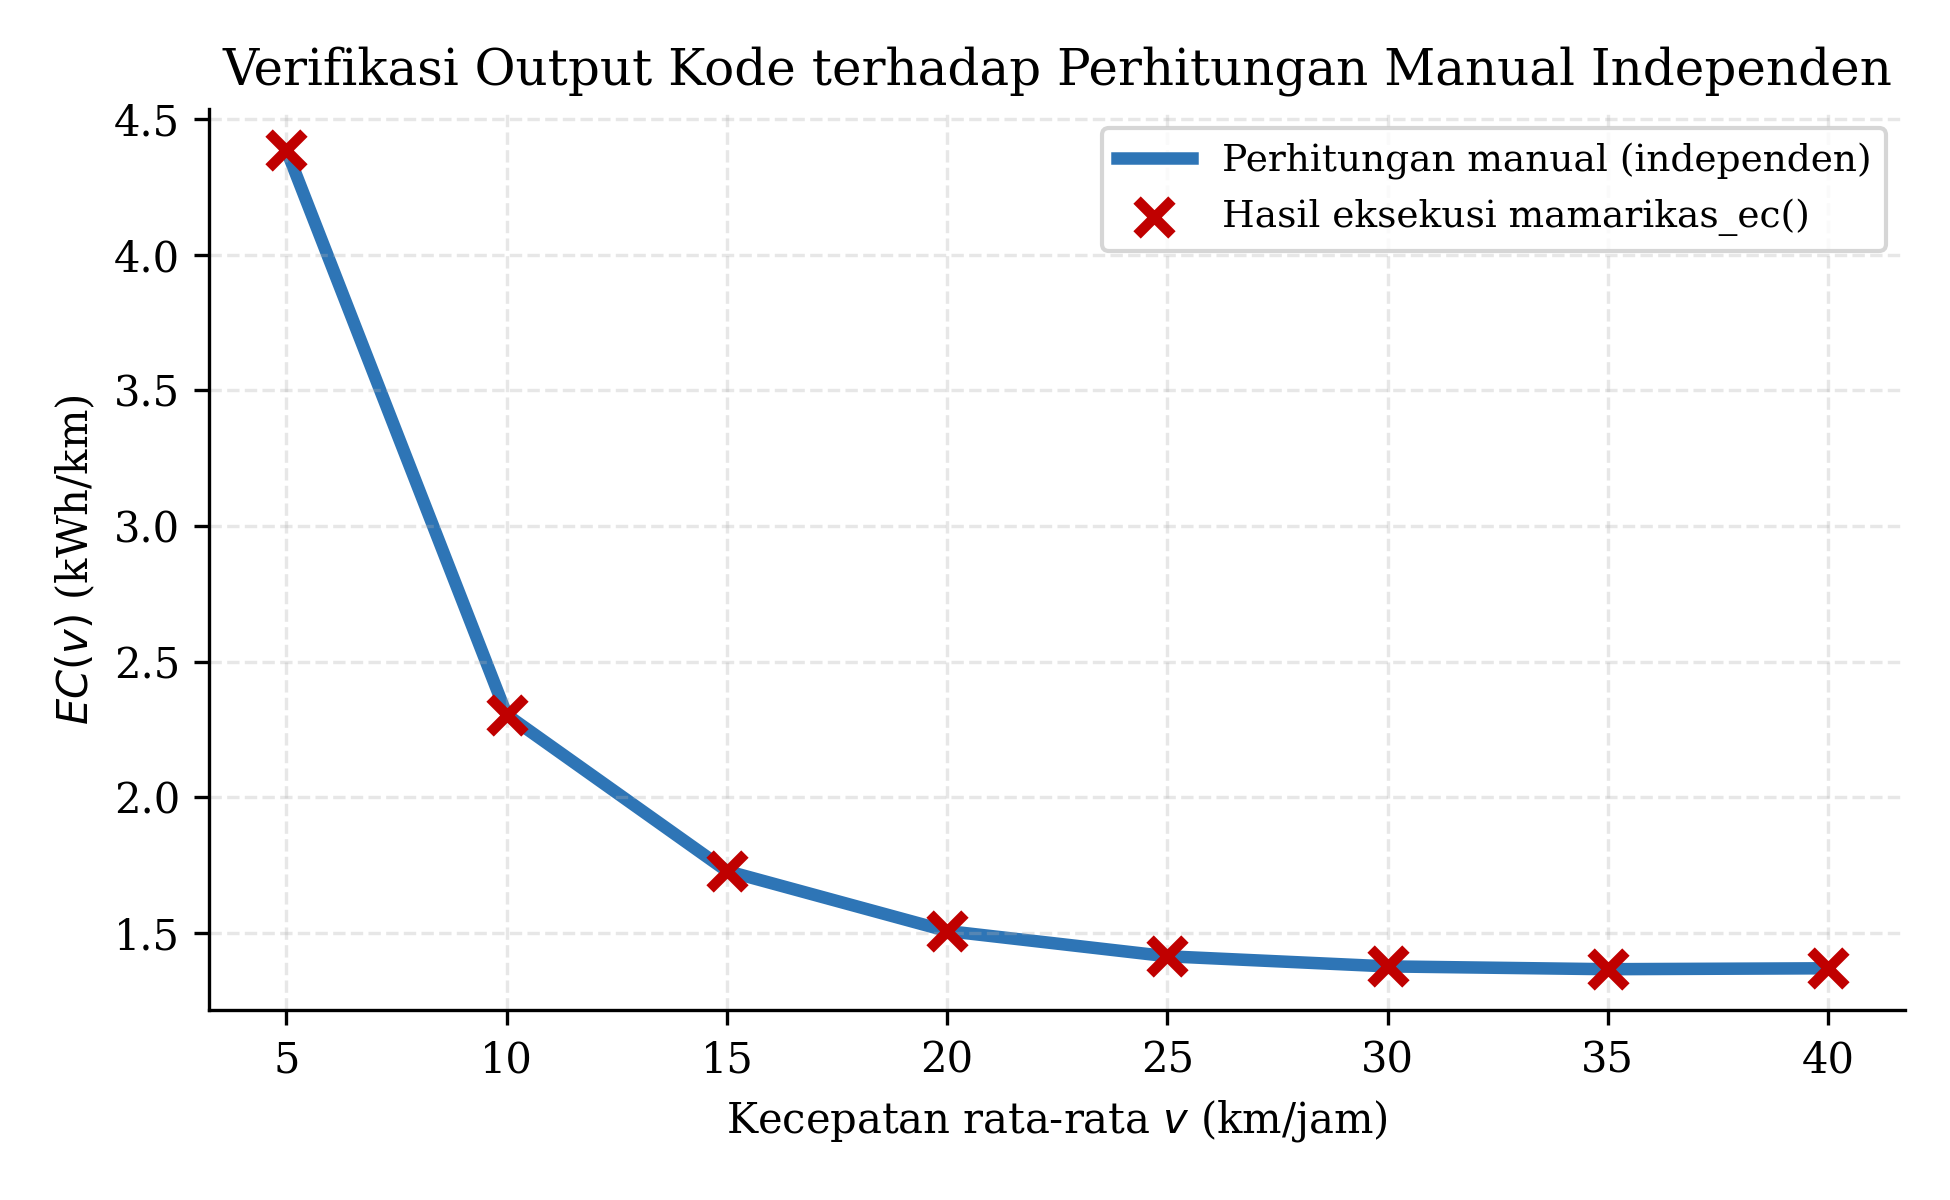
\includegraphics[width=0.75\textwidth]{images/fig_verifikasi_ecv.png}
	\caption{Verifikasi output fungsi \texttt{mamarikas\_ec()} terhadap perhitungan manual independen}
	\label{fig:verifikasi-ecv}
\end{figure}

\section{Implementasi Randomisasi Waktu Tempuh}

Randomisasi kecepatan tempuh sesuai rancangan pada Bab IV diimplementasikan
di lapisan pembungkus Monte Carlo (bukan di mesin simulasi inti), melalui
dua parameter: \texttt{daily\_time\_modifier} (dibangkitkan acak dari
\texttt{random.uniform(0.8, 1.2)} untuk tiap hari simulasi, merepresentasikan
$CV=15\%$) dan \texttt{engine.segment\_cv = 0.05} pada level segmen. Nilai
kecepatan efektif per segmen kemudian dipakai sebagai masukan fungsi
\texttt{mamarikas\_ec()} pada saat mesin simulasi dijalankan untuk hari
tersebut.

\section{Implementasi Mesin Simulasi}

Mesin simulasi diimplementasikan dalam Python (modul \texttt{simulation/engine.py})
menggunakan antrean prioritas (\texttt{heapq}) untuk memproses peristiwa 
secara kronologis. Logika utamanya dipaparkan pada Algoritma~\ref{alg:des-loop}.

\begin{algorithm}[h!]
\caption{Loop Utama Mesin Simulasi Berbasis Peristiwa Diskrit}
\label{alg:des-loop}
\begin{algorithmic}[1]
\Require Jadwal keberangkatan awal tiap bus $B$, Sumber daya SPKLU
\Ensure \textit{Trace} SoC, durasi antrean, dan jadwal keberangkatan riil
\State Inisialisasi antrean peristiwa $Q$ berbasis waktu kejadian
\For{setiap bus $b \in B$}
    \State $Q.\text{push}(\langle t_{\text{mulai}}, \text{START\_TRIP}, b \rangle)$
\EndFor
\While{$Q$ tidak kosong}
    \State $\langle t, \text{Tipe}, b \rangle \gets Q.\text{pop}()$
    \If{$\text{Tipe} == \text{START\_TRIP}$}
        \State Jalankan rit rute bus $b$, kurangi SoC di tiap segmen
        \If{SoC $\leq$ ambang batas (contoh: 30\%)}
            \State $Q.\text{push}(\langle t_{\text{tiba\_spklu}}, \text{ARRIVE\_AT\_SPKLU}, b \rangle)$
        \ElsIf{SoC $\leq 20\%$ (batas bawah aman)}
            \State Catat status bus $b$ sebagai \text{STRANDED} (mogok)
        \Else
            \State $Q.\text{push}(\langle t_{\text{selesai}}, \text{START\_TRIP}, b \rangle)$
        \EndIf
    \ElsIf{$\text{Tipe} == \text{ARRIVE\_AT\_SPKLU}$}
        \If{SPKLU penuh}
            \State Tambahkan $b$ ke antrean tunggu SPKLU
            \State Hitung ekspektasi waktu mulai cas ($t_{\text{cas}}$) dan waktu antre ($w_q$)
            \State Cek \textit{timeout}: jika $w_q \geq 30$ menit dan $t_{\text{cas}} \geq t_{\text{akhir\_shift}}$, catat \text{STRANDED}
        \Else
            \State $Q.\text{push}(\langle t + \text{durasi\_cas}, \text{FINISH\_CHARGING}, b \rangle)$
        \EndIf
    \ElsIf{$\text{Tipe} == \text{FINISH\_CHARGING}$}
        \State Bebaskan \textit{gun} SPKLU, alokasikan ke bus di antrean (jika ada)
        \State $Q.\text{push}(\langle t + \text{durasi\_kembali}, \text{START\_TRIP}, b \rangle)$
    \EndIf
\EndWhile
\end{algorithmic}
\end{algorithm}

Mesin ini mencakup lima komponen sesuai rancangan Bab IV: \texttt{BatteryDrainModel}
(drain baterai), penjadwal rit (\textit{Route/Trip Scheduler}), modul
keputusan pengisian daya (\textit{Charging Decision Module}),
\texttt{SPKLUResource} (model antrean SPKLU), dan \texttt{HeadwayEvaluator}.

\subsection{Mekanisme Pengisian Daya}

Ketiga mekanisme dasar (\textit{full opportunity}, \textit{full depot},
\textit{mix}) diimplementasikan sebagai jalur logika berbeda pada modul
keputusan pengisian daya, dipilih berdasarkan konfigurasi
\texttt{charging\_mechanism} pada berkas skenario (lihat Bab IV, Rancangan
Struktur Data Skenario).

Modul pengisian daya dinamis diimplementasikan pada fungsi
\url{compute_charge_duration()}. Pada tahap pengembangan awal modul
ini, ditemukan bahwa fungsi tersebut tidak menerima argumen
\texttt{spklu\_resource} dari pemanggil (\texttt{BusAgent.\_run\_trip()}),
sehingga varian V2 (\textit{queue-aware}, yang seharusnya membaca kondisi
antrean nyata di SPKLU tujuan) diam-diam berjalan sebagai V1
(\textit{time-aware}) tanpa terdeteksi pada pengujian awal. Perbaikan
dilakukan dengan meneruskan objek \texttt{spklu\_resource} yang relevan ke
fungsi ini saat konfigurasi \texttt{dynamic\_charging=True} dan
\texttt{dynamic\_version="v2"} aktif. Hasil pengujian kedua varian setelah
perbaikan ini dijelaskan pada Bab VI.

\subsection{Model Antrean SPKLU}

Tiap titik SPKLU diimplementasikan sebagai \texttt{SPKLUResource} dengan
kapasitas terbatas (jumlah gun) dan antrean FIFO (\textit{first-in-
	first-out}). Saat bus tiba di SPKLU dan seluruh gun terpakai, bus masuk
antrean dan menunggu hingga satu gun tersedia; durasi tunggu ini dicatat
terpisah dari durasi pengisian daya, sehingga dampak keduanya terhadap
headway dapat dianalisis secara terpisah pada Bab VI.

\section{Kalibrasi terhadap Baseline Rute L-1}

Sesuai kebutuhan nonfungsional validitas (Bab III), model drain baterai
dan mesin simulasi dikalibrasi secara kualitatif terhadap kondisi
operasional riil Rute L-1: 2 bus, 1 SPKLU di Adisucipto, dengan waktu
tidak beroperasi (\textit{downtime}) sekitar 120 menit per sesi pengisian
daya. Simulasi baseline ini disimpan sebagai
\url{simulation_result_L1.json} dengan \texttt{scenario\_id}
\url{baseline_as_is_L1_2bus_opportunity_adisucipto}, yang menjadi
acuan pembanding utama untuk seluruh skenario pada Bab VI.

Hasil kalibrasi menunjukkan bahwa mesin simulasi menghasilkan kebutuhan 3
sesi pengisian daya per hari untuk kondisi Rute L-1, sedangkan kondisi
riil di lapangan hanya memerlukan 2 sesi per hari. Deviasi ini konsisten
dengan analisis pada Bab IV: model Mamarikas dkk. (2025) dikalibrasi pada
bus kelas berat, sehingga menghasilkan estimasi konsumsi energi yang lebih
tinggi dari kondisi riil bus TransJogja. Sesuai keputusan metodologis pada
Bab III dan Bab IV, deviasi ini tidak dikoreksi dengan faktor skala buatan,
melainkan diterima dan dicatat sebagai batasan akurasi model.

\section{Implementasi Simulasi Monte Carlo}

Simulasi Monte Carlo diimplementasikan sebagai lapisan pembungkus di luar
mesin simulasi inti. Pembungkus ini bertugas menjalankan mesin simulasi
berulang kali (sejumlah $N$ hari) untuk setiap skenario, masing-masing dengan
kecepatan tempuh dasar yang dirandomisasi secara global pada awal setiap iterasi, 
seperti diilustrasikan pada Algoritma~\ref{alg:monte-carlo}.

\begin{algorithm}[h!]
\caption{Pembungkus Simulasi \textit{Monte Carlo} Multi-hari}
\label{alg:monte-carlo}
\begin{algorithmic}[1]
\Require Jumlah iterasi hari $N$, Definisi skenario operasional $S$
\Ensure Metrik kinerja operasional rata-rata dan standar deviasi
\State Inisialisasi koleksi $R \gets \emptyset$ untuk menyimpan hasil harian
\For{$i = 1$ \textbf{to} $N$}
    \State Bangkitkan \textit{modifier} kemacetan harian $M_{\text{daily}}$ (distribusi \textit{log-normal})
    \State Set SoC awal = 100\% untuk semua armada bus
    \State Jalankan \textbf{Algoritma~\ref{alg:des-loop}} dengan \textit{modifier} hari ke-$i$
    \State Simpan metrik harian (rute lumpuh, rata-rata \textit{headway}) ke dalam $R$
\EndFor
\State Hitung $\mu$ dan $\sigma$ dari distribusi sampel di dalam $R$
\State \Return Statistik agregat simulasi
\end{algorithmic}
\end{algorithm}

Proses ini menangkap variasi hari-ke-hari seperti kemacetan atau kelancaran
lalu lintas sistemik. Hasil akhir untuk setiap skenario bukan berupa satu
hari simulasi, melainkan agregasi statistik dari $N$ hari, berdasarkan
pengujian konvergensi $N=50$ dibanding $N=100$ terhadap metrik headway
rata-rata, sesuai rancangan pada Bab IV.

Hasil tiap repetisi harian disimpan sebagai data mentah per skenario
(\url{<scenario_id>_daily_route_gaps.json}), kemudian diagregasi
menjadi ringkasan statistik (rata-rata dan deviasi standar) pada
\url{data/comparison_table_stochastic.csv}, yang menjadi dasar
perbandingan antar-skenario pada Bab VI.

\section{Implementasi Dasbor Visual}

Dasbor visual diimplementasikan sebagai aplikasi Flask yang menyajikan
hasil simulasi (berkas JSON per skenario) melalui API, dikonsumsi oleh
\textit{frontend} HTML/JavaScript murni. Peta skematik rute dibangun
sebagai SVG generatif dari data urutan halte tiap koridor, dengan peta
rute resmi TransJogja sebagai referensi visual pembanding. Chart.js
dipakai untuk menampilkan grafik metrik hasil (headway, tingkat kegagalan
rute) pada panel metrik.

Gambar~\ref{fig:dashboard-overview} menunjukkan tampilan dasbor saat
menampilkan seluruh 20 koridor pada skenario S34, mencakup peta skematik
rute, panel kontrol simulasi (pemilihan skenario, kecepatan pemutaran),
panel perbandingan seluruh skenario, dan grafik SoC seluruh armada bus.

\begin{figure}[h]
	\centering
	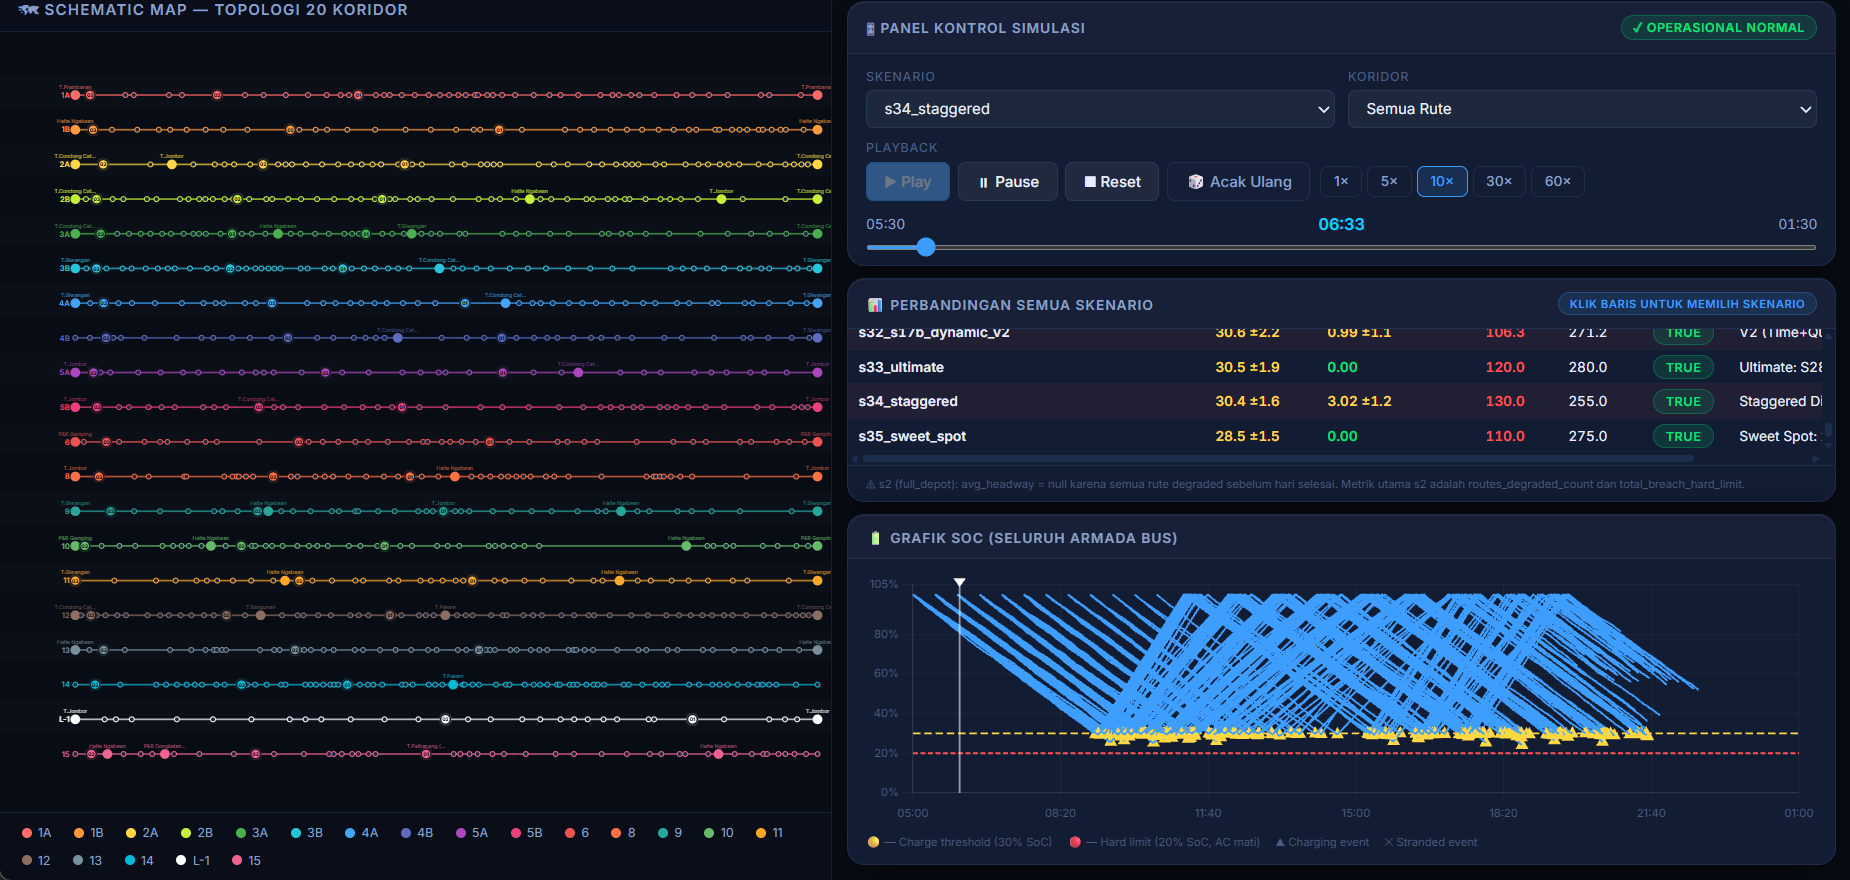
\includegraphics[width=\textwidth]{images/dashboard_peta_skematik.png}
	\caption{Tampilan dasbor visual: peta skematik 20 koridor dan panel perbandingan skenario}
	\label{fig:dashboard-overview}
\end{figure}

Dasbor juga mendukung penyaringan tampilan per koridor. Gambar~\ref{fig:dashboard-filter}
menunjukkan tampilan saat koridor Rute L-1 dipilih: rute lain diredupkan
pada peta skematik, dan grafik SoC hanya menampilkan 2 bus yang beroperasi
pada rute tersebut, mempermudah penelusuran perilaku SoC pada satu
koridor tertentu.

\begin{figure}[h]
	\centering
	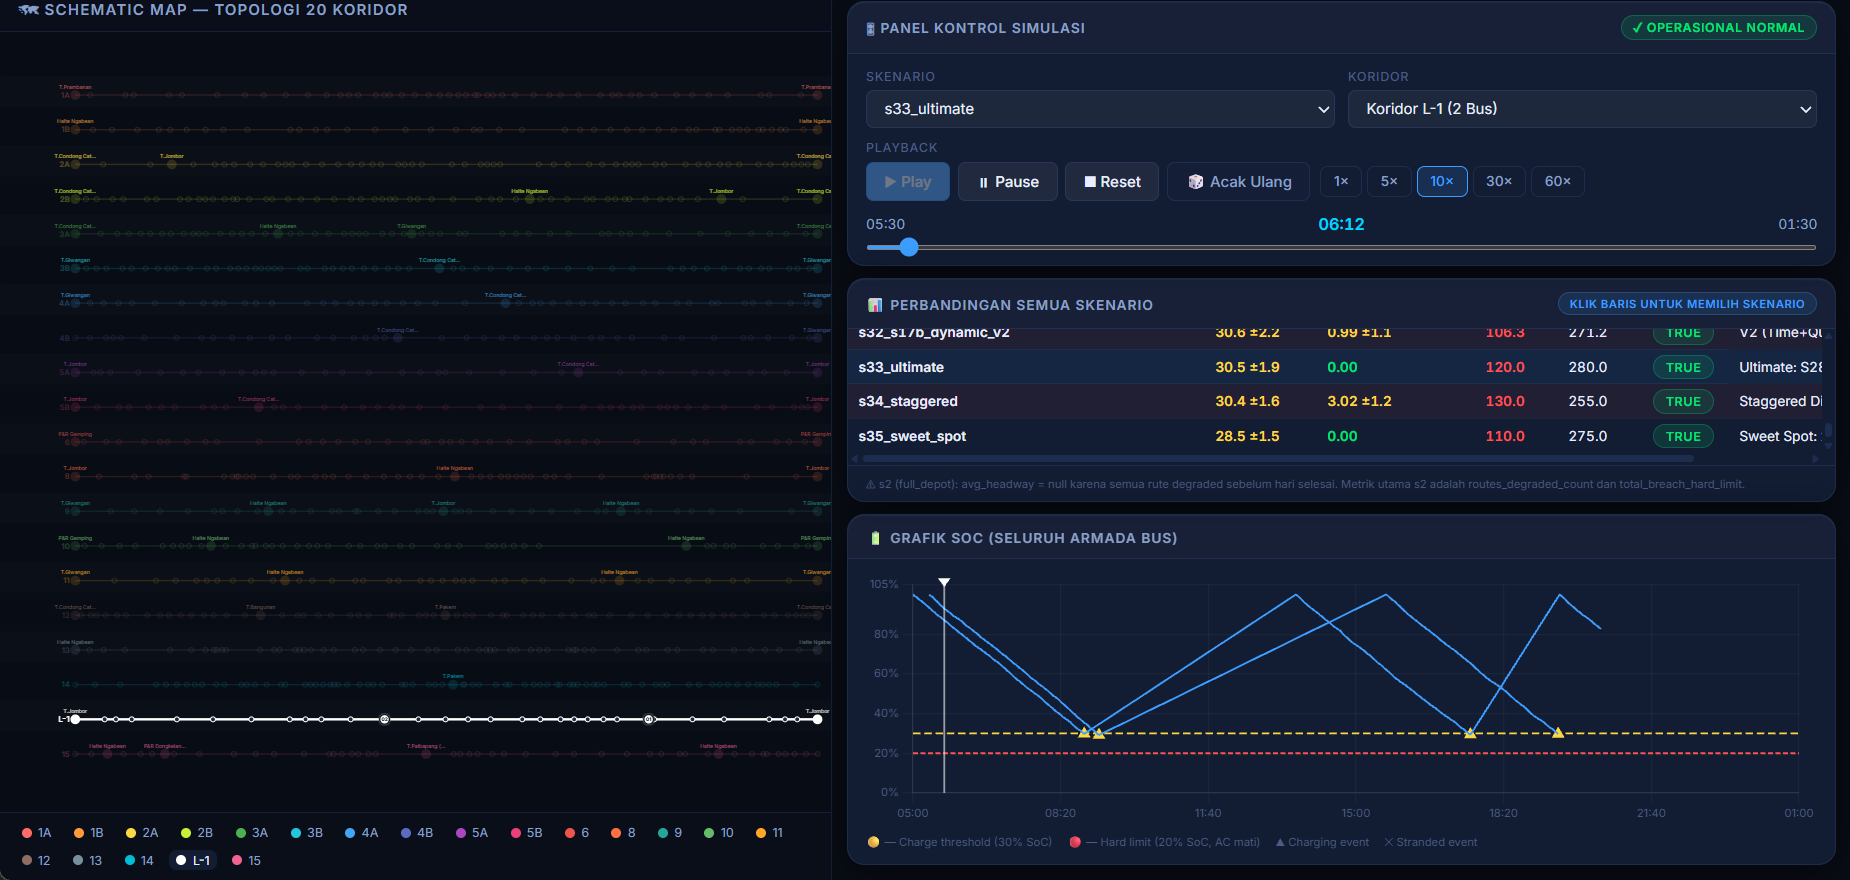
\includegraphics[width=\textwidth]{images/dashboard_playback_detail.png}
	\caption{Tampilan dasbor saat menyaring per koridor (Rute L-1, skenario S33)}
	\label{fig:dashboard-filter}
\end{figure}

\textit{Backend} memuat berkas hasil simulasi secara \textit{lazy}
(\textit{lazy-load}), yaitu hanya membaca berkas JSON skenario yang
sedang diminta oleh \textit{frontend}, bukan memuat seluruh hasil simulasi
ke memori sekaligus saat aplikasi dijalankan. Pendekatan ini konsisten
dengan kebutuhan nonfungsional keterpisahan (Bab III): \textit{backend}
tidak menjalankan ulang logika simulasi, hanya menyajikan data yang sudah
tersimpan.